\section{Challenges}\label{sec:challenges}

Politou et al.~\cite{Politou2017} discussed most of the challenges in smartphone affective research which covers \emph{privacy}, \emph{data misuse}, \emph{trust and engagement}, \emph{multimodal fusion}, \emph{resource constraints}, \emph{affect modelling and representation}, \emph{cultural differences} and \emph{system building costs}. From the technique prespective, challenges and limitations can be summarized to the following sections.

\subsection{Impermeable Emotions}

The primary limitation of traditional affective computing research refers to as impermeable emotions~\cite{picard2003affective}. Impermeable emotions are broad, with many of these modalities being inaccessible (e.g., blood chemistry, brain activity, neurotransmitters), and many others being too non-differentiated. It makes it unlikely that collecting the necessary data will be possible or feasible in the near future. 

There is a time period to express emotion, and a time period to forbear; a time period to sense what others are feeling and a time period to ignore feelings. In every time, human need a balance when they express their emotions, and this balance is missing in computing. Figure~\ref{fig:emotions} illustrates a map of human emotions. The largest text represents the most expressible emotions and the arrow in the graph indicates how emotions related to each other, which is can be consider as a analogy of Markov chain.
The all recent classification method doesn't provides this consideration. A close look to the smaller text in this picture, almost all of them are impermerable emotions that can never be discovered by emotion inference model since can not be labeled in a dataset.

In most cases, researchers feel positive and argue that impermeable emotions can be expressed explicitly in other expressed Emotions~\cite{parkinson1995ideas} and implicit emotions are trivial and not crucial for most of the case of affective computing application when we need an emotion state~\cite{Zhang2014}. However, impermeable emotion is still an open problem and challenging research area in affective computing.

\begin{figure}[htb]
    \centering
    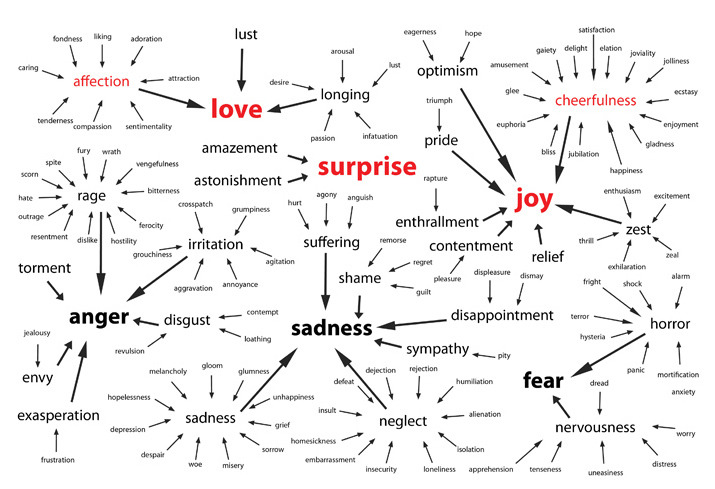
\includegraphics[width=3.5in]{emotion-map}
    \caption{A map of human emotions. Image from~\cite{emotionmap}.}
    \label{fig:emotions}
\end{figure}


\subsection{Continious Understanding}

Emotions are not states. Continuous emotion understanding is much more challenging since it's not related to external emotion but also related to internal emotions; various emotions can be expressed as the map \textit{(see Figure~\ref{fig:emotions})} we discussed above.

Most of the researchers we introduced in the previous section treated emotion inference problem as a classification problem, whereas the human emotions are always passive and instantaneous. People's expression of emotion is so idiosyncratic and variable, that there is little hope of accurately recognizing an individual’s emotional state from the available data sometimes.

\subsection{Context Specific Models}

A potential ethical limitation in research studies comes from the fact that perceptions of emotions and personality are not universal, but they are highly dependent on the mobile application context~\cite{Gao2012, Shah2015, bhattacharya2017predictive, Tikadar2017} as well as the cultural differences between humans~\cite{mesquita1992cultural, masuda2008placing, gendron2014perceptions}. According to these perspectives, a reasonable challenge is how an affective recognition model should be designed and built in an application and transparent cultural way.

\subsection{Lack of Computation Resources}

As we discussed before, CNN and depth camera methods require large computation resource. 
Apparently, computation resources are limited in a mobile device. Consequently, an issue that impacts the effectiveness of emotion inference system is the fusion of all kinds of multimodal.

To handling such informations in run-time, for mobile devices with limited operation time and processing power is not possible. Cloud computing is a way of sending processing data from mobile device to powerful server, it significantly mitigates the computation stress of a mobile device but also increases the delay of emotion inference due to communication delay between server and mobile phone.
